\documentclass[12pt, letterpaper, twoside]{article}
\usepackage[utf8]{inputenc}
\usepackage{listings}
\usepackage{color}
\usepackage{graphicx}

\graphicspath{ {./images/} }

\definecolor{dkgreen}{rgb}{0,0.6,0}
\definecolor{gray}{rgb}{0.5,0.5,0.5}
\definecolor{mauve}{rgb}{0.58,0,0.82}

\lstset{frame=tb,
  aboveskip=2mm,
  belowskip=2mm,
  showstringspaces=false,
  columns=flexible,
  basicstyle={\small\ttfamily},
  numbers=left,
  numberstyle=\tiny\color{gray},
  keywordstyle=\color{blue},
  commentstyle=\color{dkgreen},
  stringstyle=\color{mauve},
  breaklines=true,
  breakatwhitespace=true,
  tabsize=2
}

\title{%
Design and Analysis of Algorithms\\
\large 5.3 Linear Programming
}
\author{Daniel Shannon}
\date{May 5th, 2022}

\begin{document}

\begin{titlepage}
\maketitle
\end{titlepage}

\section*{5.3.2}

\begin{quote}
  \begin{itemize}
    \item You have a store that makes and sells calculators.
    \item Demand tells you to produce at least 100 scientific calculators and 80 graphing calculators per day.
    \item You can make at most 200 scientific calculators and 170 graphing calculators each day.
    \item Because of a contract, you must produce at least 200 calculators per day.
    \item Each scientific calculator gives you a \$2 loss, and each graphing calculator gives you a \$5 profit.    
  \end{itemize}
  Formulate this as a linear programming problem
\end{quote}

\begin{itemize}
  \item $x_0$ scientific calculator
  \item $x_1$ graphing calculator
  \item $p$ profit
\end{itemize}

$$100\le{}x_0\le{}200$$
$$80\le{}x_1\le{}170$$
$$x_0+x_1\ge{}200$$
$$p=-2x_0+5x_1$$

\newpage
\section*{5.3.5}

\begin{quote}
  Find the maximum amount of flow from s to t.
  \begin{center}
    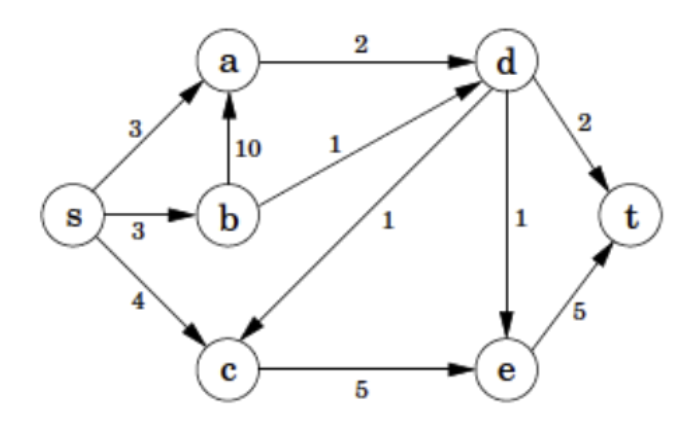
\includegraphics{5_3_5.png}
  \end{center}  
\end{quote}

$$MAX(sa+ad+dt+sc+ce+et+5sb+3ba+2bd+2de+2dt+2et)$$
$$sa+ad+dt\le{2}$$
$$sc+ce+et\le{4}$$
$$sb+ba+ad+dt\le{1}$$
$$sb+ba+bd+dt\le{1}$$
$$sb+ba+ad+de+et\le{1}$$
$$sb+bd+de+et\le{1}$$
$$sb+bd+dc+ce+et\le{1}$$

Max flow is 6.

\newpage
\section*{5.3.7}
\begin{quote}
  \begin{itemize}
    \item There are $k$ factories that produce up to $g_1$, ..., $g_k$
    \item There are $n$ warehouses that can store up to $w_1$, ..., $w_n$ quantity of goods. (Assume integers.)
    \item A factory can supply a warehouse if they are within 100 miles of each other.
    \item What is the maximum number of goods that can be stored?
  \end{itemize}
\end{quote}
\begin{center}
  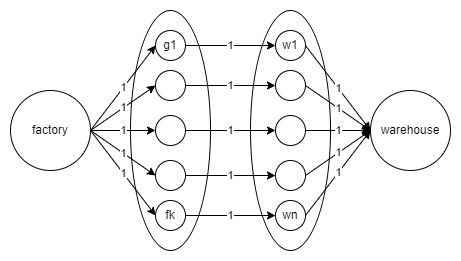
\includegraphics[scale=.75]{5_3_7_biparate_graph.png}
\end{center}
$$g_k-w_n\le{100}$$
$$g_k-w_n+s=100$$

\newpage
\section*{5.3.9}
\begin{quote}
  Suppose that in addition to a maximum capacity on edges, each node has a demand: a certain amount of flow that it will use up. How do we find if there is a feasible flow?
\end{quote}

Since the outflow is now dependent on the rate of inflow and consumption, I would take find the maximum
of rate.
$$max[(r_{in}-c_{node}r_{node}\le{c_{out}})\frac{d}{dr}]$$
\end{document}
